\subsubsection{Ping}
\paragraph{Shell}
\begin{lstlisting}[language=Bash, caption=Ping Google Public DNS]
$ ping 8.8.8.8 -c 2
PING 8.8.8.8 (8.8.8.8) 56(84) bytes of data.
64 bytes from 8.8.8.8: icmp_seq=1 ttl=116 time=22.6 ms
64 bytes from 8.8.8.8: icmp_seq=2 ttl=116 time=19.6 ms

--- 8.8.8.8 ping statistics ---
2 packets transmitted, 2 received, 0% packet loss, time 1002ms
rtt min/avg/max/mdev = 19.639/21.124/22.610/1.485 ms
\end{lstlisting}
\paragraph{Wireshark}
\begin{figure}[!htb]
    \centering
    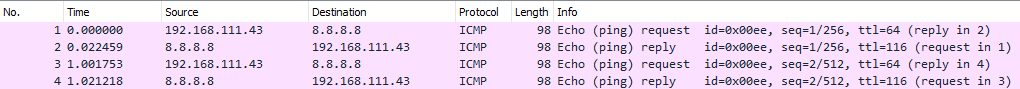
\includegraphics[width=\textwidth,height=.85\textwidth,keepaspectratio]{./img/echo_reply_request.png}
    \caption{Erweitertes Netzwerk}
\end{figure}
\FloatBarrier
Wie erwartet gingen 2 Echo-requests raus und es kamen 2 Echo-replies an.
\subsubsection{Ping mit Fragmentation}
\paragraph{Shell}
\begin{lstlisting}[language=Bash, caption=Linux ping with More Fragment]
$ ping 8.8.8.8 -s 1500
PING 8.8.8.8 (8.8.8.8) 1500(1528) bytes of data.
^C
--- 8.8.8.8 ping statistics ---
3 packets transmitted, 0 received, 100% packet loss, time 2078ms
\end{lstlisting}
\begin{lstlisting}[language=Bash, caption=Window ping with More Fragment]
$ ping 8.8.8.8 -l 1500

Pinging 8.8.8.8 with 1500 bytes of data:
Request timed out.
Request timed out.

Ping statistics for 8.8.8.8:
    Packets: Sent = 2, Received = 0, Lost = 2 (100% loss),
Control-C
\end{lstlisting}
\noindent
Das Ergebnis ist wie erwatet, denn die Daten dürfen nur 1472 bytes groß sein, da Ethernet maxmial 1500 Bytes (1518 mit Header und FCS) erlaubt. Der Grund dafür ist, dass der IP Header 20 Bytes und der ICMP Header 8 Bytes ist. 1500 - 28 = 1472.\\
Der More Fragment Header war jedoch gesetzt, aber die meisten Provider, Server, Router, etc., blocken ICMP fragmentation aus historischen Gründen und weil fragmentation keine Paketverluste erlaubt, ansonsten kann das Paket nicht zusammengesetzt werden.\\
Da mein lokales Netzwerk dies jedoch nicht hat, kann ich Pakete mit dem DF flag senden und bekomme eine Antwort zurück.
\paragraph{Wireshark}
\begin{figure}[!htb]
    \centering
    \begin{subfigure}{.6\textwidth}
        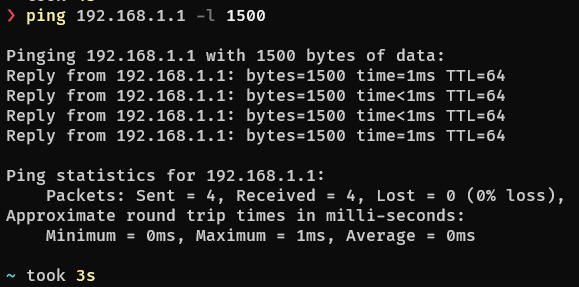
\includegraphics[width=\textwidth]{./img/MF_ping.png}
        \caption{Terminal}
    \end{subfigure}
    \begin{subfigure}{\textwidth}
        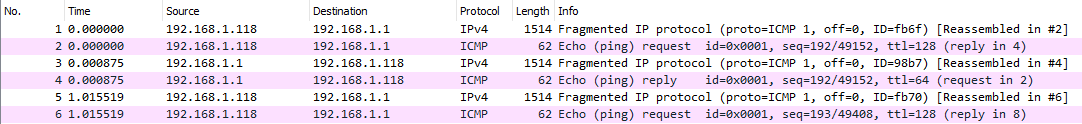
\includegraphics[width=\textwidth,height=\textwidth,keepaspectratio]{./img/MF_ping_WS.png}
        \caption{Wireshark Trace}
    \end{subfigure}
    \caption{Ergebnisse}
\end{figure}
\FloatBarrier

\subsubsection{Traceroute\textbackslash Tracert}
\paragraph{Shell}
\begin{lstlisting}[language=Bash, caption=Linux traceroute]
$ traceroute -m 1 8.8.8.8 
traceroute to 8.8.8.8 (8.8.8.8), 1 hops max, 60 byte packets
 1  DESKTOP-DJVEGIR (192.168.96.1)  0.211 ms  0.216 ms  0.214 ms
\end{lstlisting}
\begin{lstlisting}[language=Bash, caption=Darwin traceroute]
$ traceroute -m 1 8.8.8.8 
traceroute to 8.8.8.8 (8.8.8.8), 1 hops max, 60 byte packets
 1  192.168.1.1 (192.168.1.1)  0.211 ms  0.216 ms  0.214 ms
\end{lstlisting}
\begin{lstlisting}[language=Bash, caption=Windows tracert]
$ tracert -h 1 8.8.8.8
Tracing route to dns.google [8.8.8.8]
over a maximum of 1 hops:
1    <1 ms    <1 ms    <1 ms  192.168.1.1
Trace complete.    
\end{lstlisting}
\paragraph{Wireshark}
\begin{figure}[!htb]
    \centering
    \begin{subfigure}{\textwidth}
        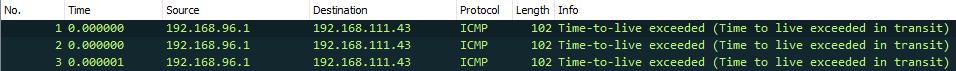
\includegraphics[width=\textwidth,height=.85\textwidth,keepaspectratio]{./img/linux_traceroute.png}
        \caption{Linux}
    \end{subfigure}
    \begin{subfigure}{\textwidth}
        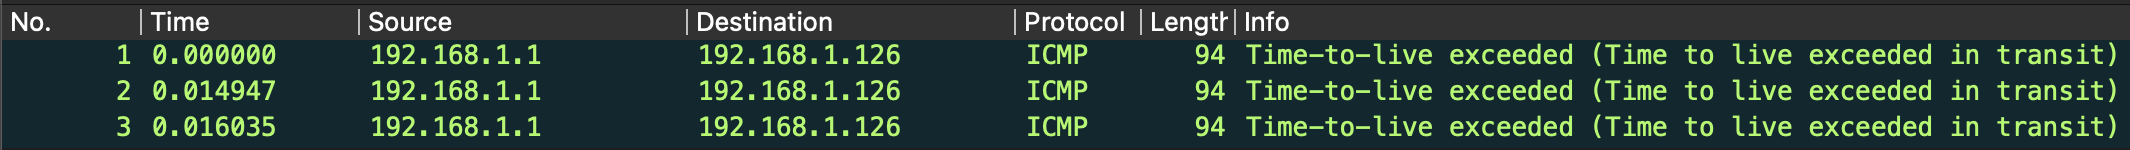
\includegraphics[width=\textwidth,height=.85\textwidth,keepaspectratio]{./img/darwin_traceroute.png}
        \caption{Darwin}
    \end{subfigure}
    \begin{subfigure}{\textwidth}
        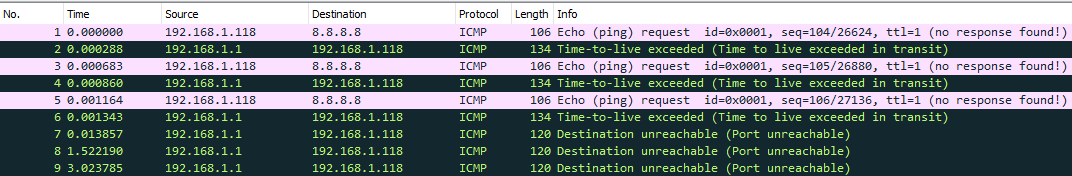
\includegraphics[width=\textwidth,height=.85\textwidth,keepaspectratio]{./img/windows_tracert.png}
        \caption{Windows}
    \end{subfigure}
    \caption{Traceroute auf den verschieden Betriebssystemen}
\end{figure}
\noindent
Da Darwin und Linux auf Unix basieren,haben beide den gleichen traceroute und wie erwartet enstand ein ttl exceeded. Es werden immer 3 Packets gesendet, damit man einen Durchschnitt hat.\\
Windows tracert verhält sich jedoch anders und sendet ein Echo-request bei einem Traceroute raus. Da der echo nie die Destination erreicht, bekommt man zusätzlich zu ttl exceeded auch ein Destination unreachable(Port unreachable)